\rhead{Path Planning}

\chapter{Path Planning}
\label{sec:path_planning}

\begin{figure}[!h]
\centering
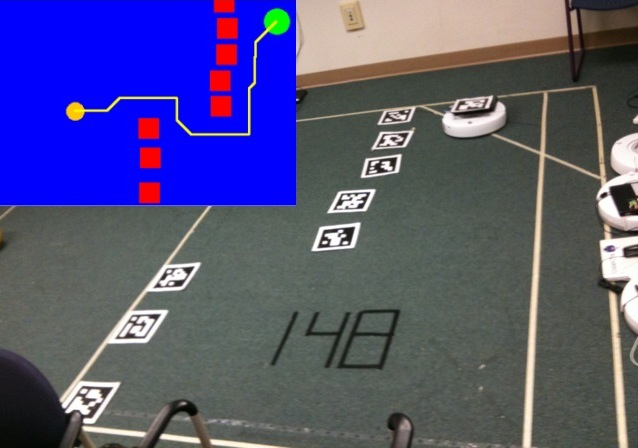
\includegraphics[width=1.0\columnwidth]{figures/7_teaser.jpg}
\end{figure}

\newpage

% \bkorel{retake teaser image with same setup but ball in the goal position}

Given a map of the field and an overhead camera view of the robots, develop a deliberative planning-based robot client for visiting specific locations and pushing a ball into a goal.

\section{Introduction}

\begin{wrapfigure}{r}{.37\columnwidth}
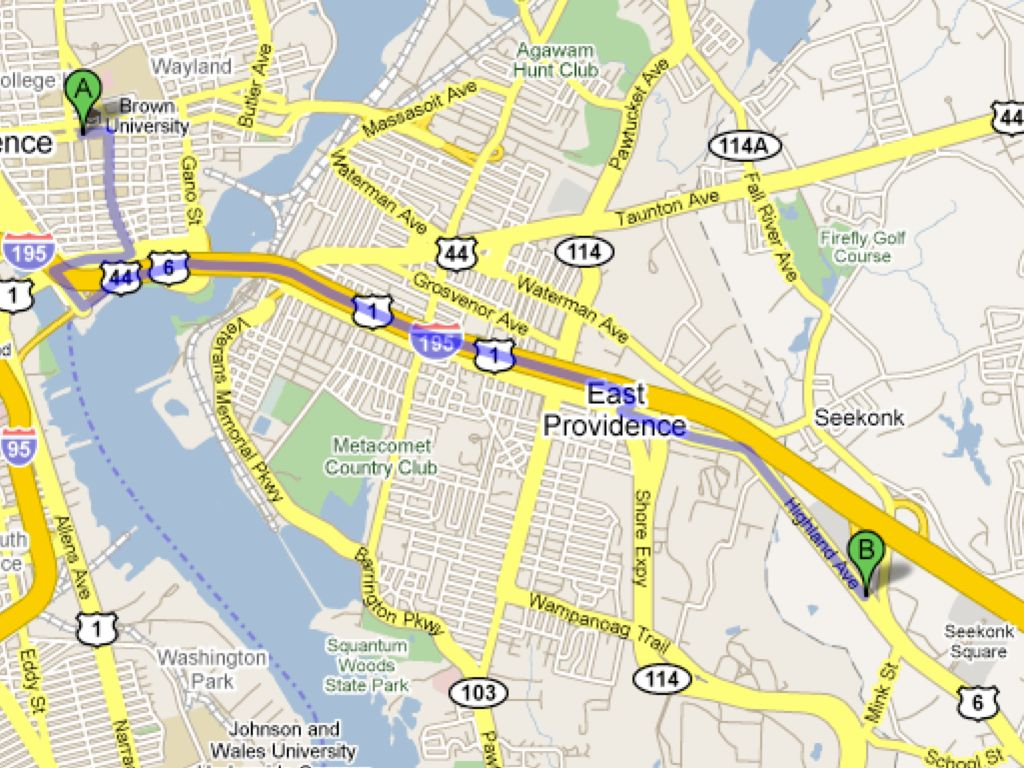
\includegraphics[width=0.35\columnwidth]{figures/7_googlemaps.jpg}
\end{wrapfigure}

With our introduction to PSG in assignments 1 and 2 behind us, it is now time to dig into making our robots play soccer.  The next four projects will follow different approaches to autonomous robot control for 1-on-1 soccer through deliberation, state estimation, reaction, and learning.  In the current assignment, you will use path planning algorithms to control your robot soccer player using overhead sensing.  In class, we will cover several different planning algorithms that you can choose from for your implementation.  Your planner implementation within your control client will be providing updated game state and the static dimensions of the field.  You will evaluate your client through basic skills challenges such as navigating to specific locations, and competition against other groups.

\section{Key Concepts}

For this project, your client will deliberatively plan and navigate paths for the robot.  At its core, this client must be able to maneuver the robot from its current pose, expressed as the position and orientation triplet $X = (x,y,\theta)$, to reach a desired destination, also expressed as pose $X' = (x',y',\theta')$.  A sequence of destinations can then form a trajectory for the robot to traverse.   An estimate of the current robot pose is provided by a state estimation system from robot sensing given a map of the environment through a process called {\it localization}.  In this assignment, localization is performed external to the robot using overhead cameras.  The map of the soccer field is described in the following section.  This setup will allow us to focus mostly on the planning problem, whereas the next assignment deals strictly with localization from onboard robot sensing.  Note: even though a localization mechanism is provided, it is neither precise nor deterministic.  Be careful to process state estimates with some considerations of uncertainty.

Given localization, a map, and a goal destination, you must plan and traverse a path from your current location to the goal.  Planning is essentially a search over all possible routes from $X$ to $X'$, or configuration space.  Graphs are typically used to express the space of possible poses (as graph vertices) and valid transitions between poses (as graph edges).  Your robot client will need to construct graphs in the robot's configurations space and then search this graph to find good paths to traverse.  For planning algorithms you have a number of options:

\begin{itemize}
\item \href{http://en.wikipedia.org/wiki/Dijkstra\%27s\_Algorithm}{Dijkstra's Algorithm}\footnote{http://en.wikipedia.org/wiki/Dijkstra\%27s\_Algorithm}, 
\item \href{http://en.wikipedia.org/wiki/A\%2A\_search}{A*}\footnote{http://en.wikipedia.org/wiki/A\%2A\_serach}
\item Potential fields (Choset Ch. 4) and \href{http://playerstage.sourceforge.net/doc/Player-2.0.0/player/classPlayerCc\_1\_1PlannerProxy.html}{Wavefront planning}\footnote{http://playerstage.sourceforge.net/doc/Player-2.0.0/player/classPlayerCc\_1\_1PlannerProxy.html}
\item Probablistic roadmaps [1] (Kavraki et al. 1996) 
\item RRT-Connect [2] (Kuffner et al. 2000)
\end{itemize}

\begin{figure}[!h]
\centering
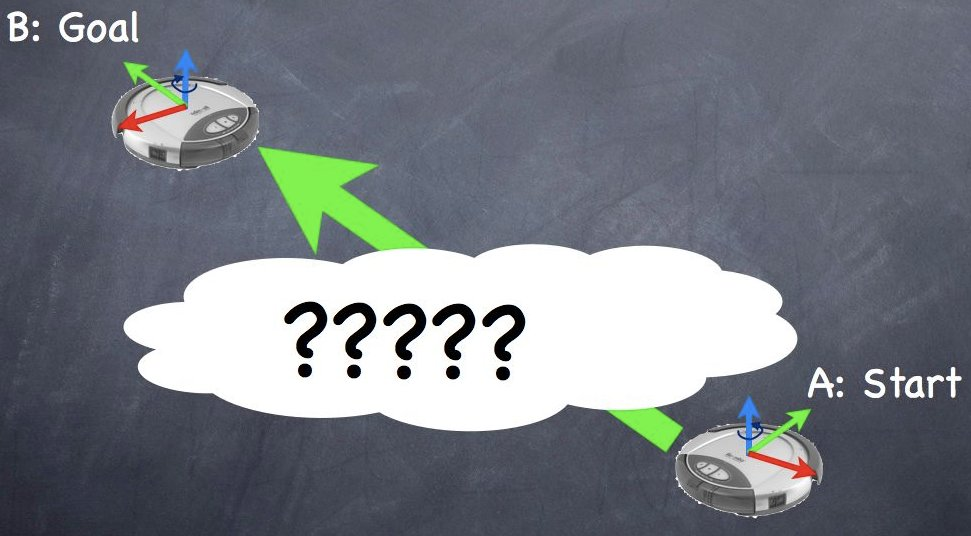
\includegraphics[width=0.6\columnwidth]{figures/7_planning1.jpg}
\caption{How to get from A to B?}
\end{figure}

\begin{figure}[!h]
\centering
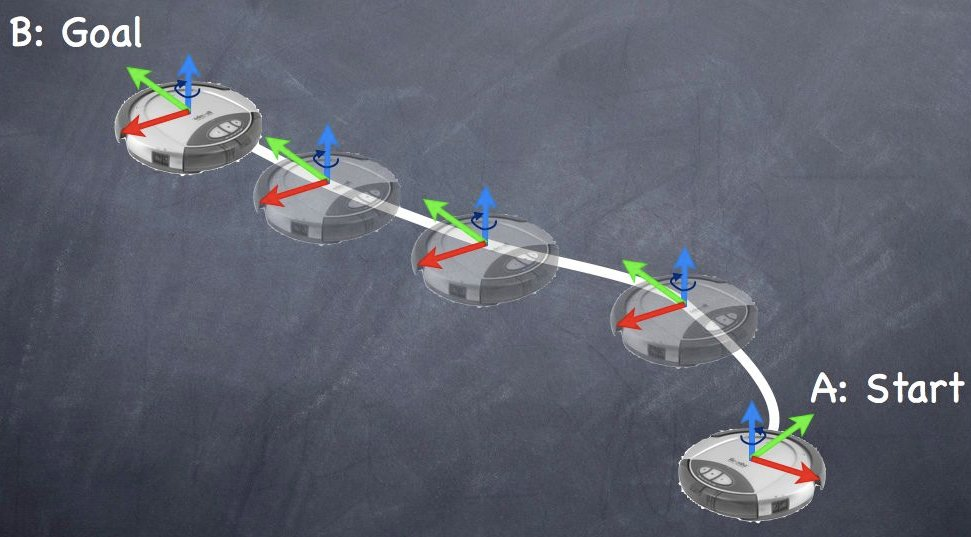
\includegraphics[width=0.6\columnwidth]{figures/7_planning2.jpg}
\caption{Path Planning}
\end{figure}

\begin{figure}[!h]
\centering
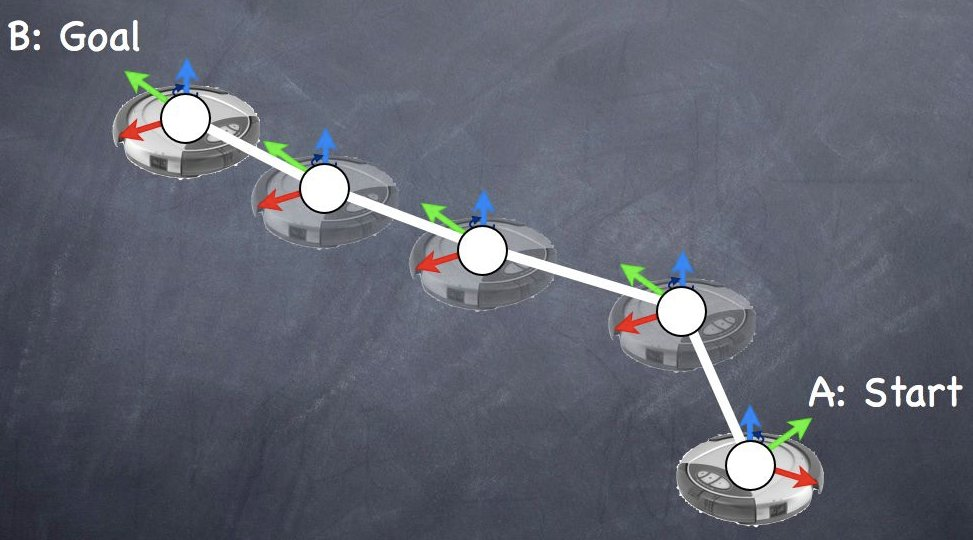
\includegraphics[width=0.6\columnwidth]{figures/7_planning3.jpg}
\caption{Path Planning}
\end{figure}

\begin{figure}[!h]
\centering
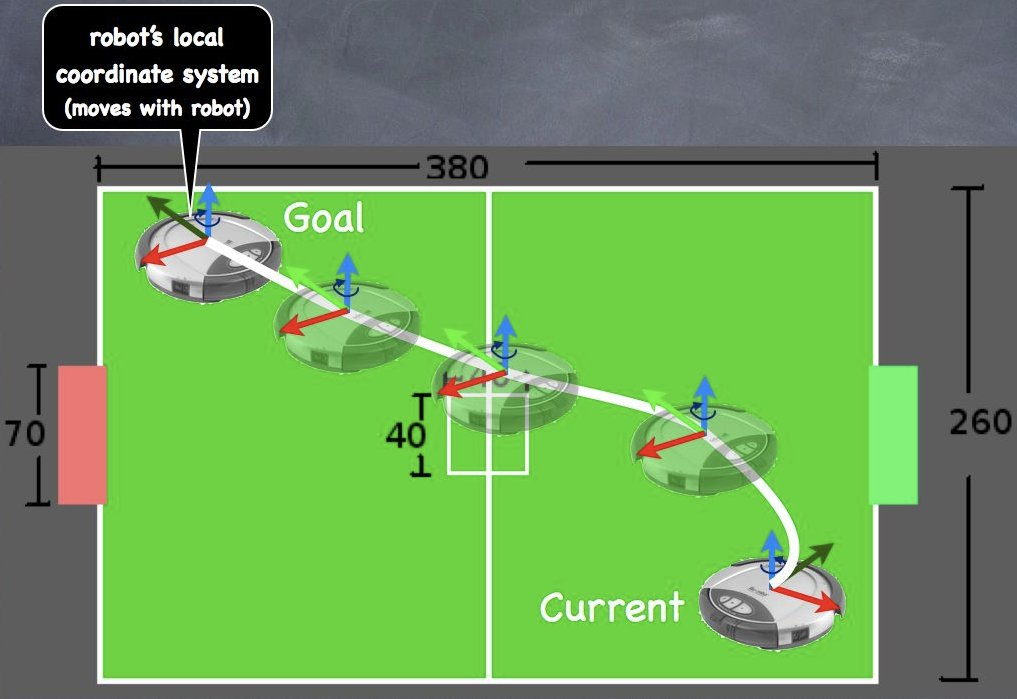
\includegraphics[width=0.6\columnwidth]{figures/7_planning4.jpg}
\caption{Path Planning}
\end{figure}

\begin{figure}[!h]
\centering
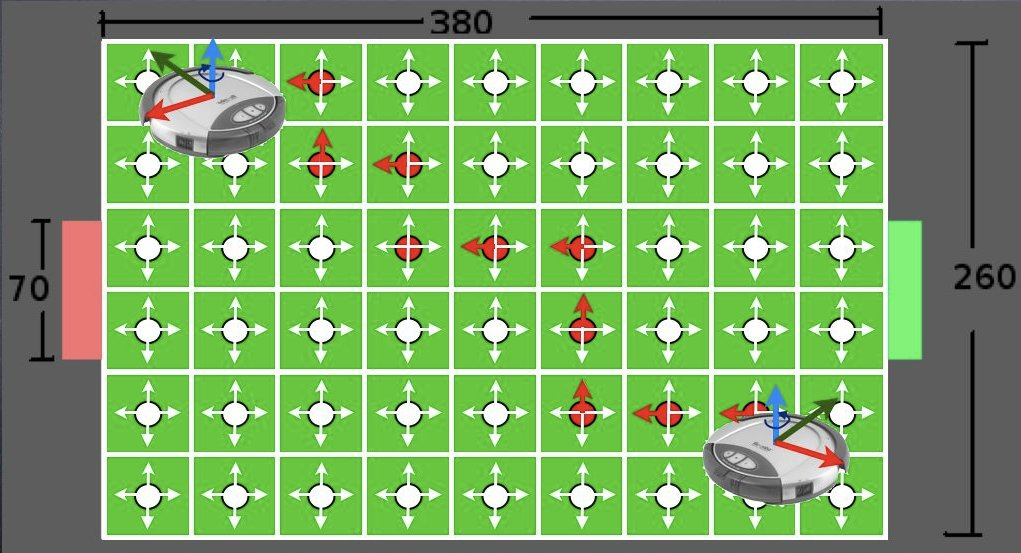
\includegraphics[width=0.6\columnwidth]{figures/7_planning5.jpg}
\caption{Poses as graph vertices connected by adjacent edges}
\end{figure}


\subsection{Dijkstra and A* Search}

\begin{figure}
\centerline{
\mbox{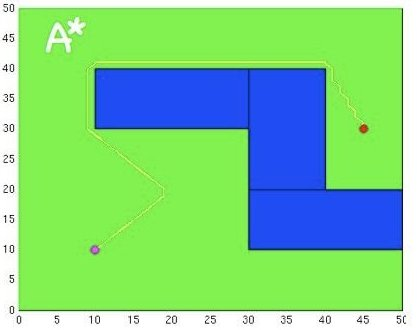
\includegraphics[width=2.10in]{figures/7_grid1.jpg}}
\mbox{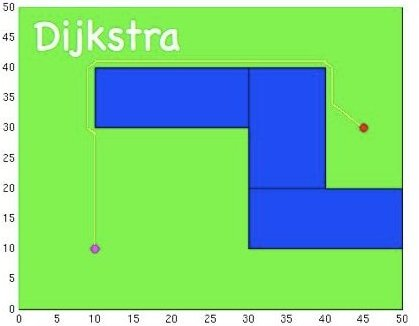
\includegraphics[width=2.10in]{figures/7_grid2.jpg}}
\mbox{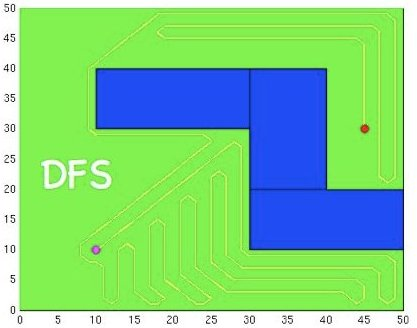
\includegraphics[width=2.10in]{figures/7_grid3.jpg}}
}
\caption{Grid Search Algorithms}
\end{figure}

link: A* Matlab Demo

\subsection{Potential Fields}

\begin{figure}[!h]
\centering
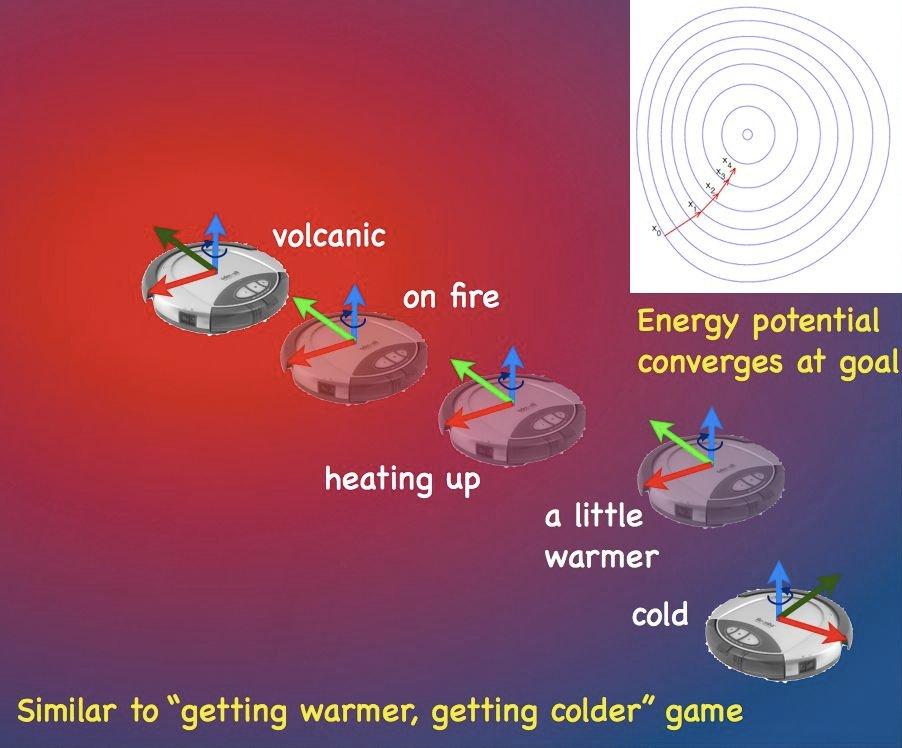
\includegraphics[width=0.6\columnwidth]{figures/7_potential1.jpg}
\caption{Potential Fields}
\end{figure}

\begin{figure}[!h]
\centering
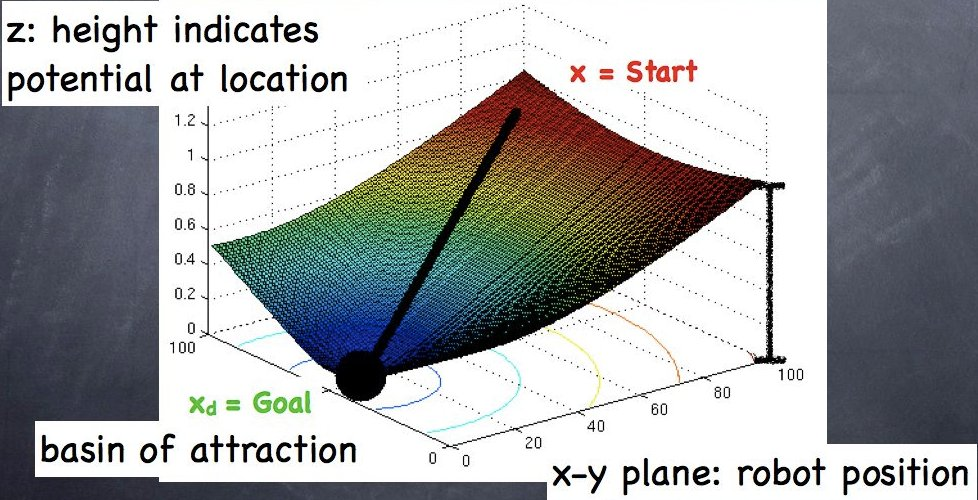
\includegraphics[width=0.6\columnwidth]{figures/7_potential2.jpg}
\caption{2D potential navigation}
\end{figure}

\begin{figure}[!h]
\centering
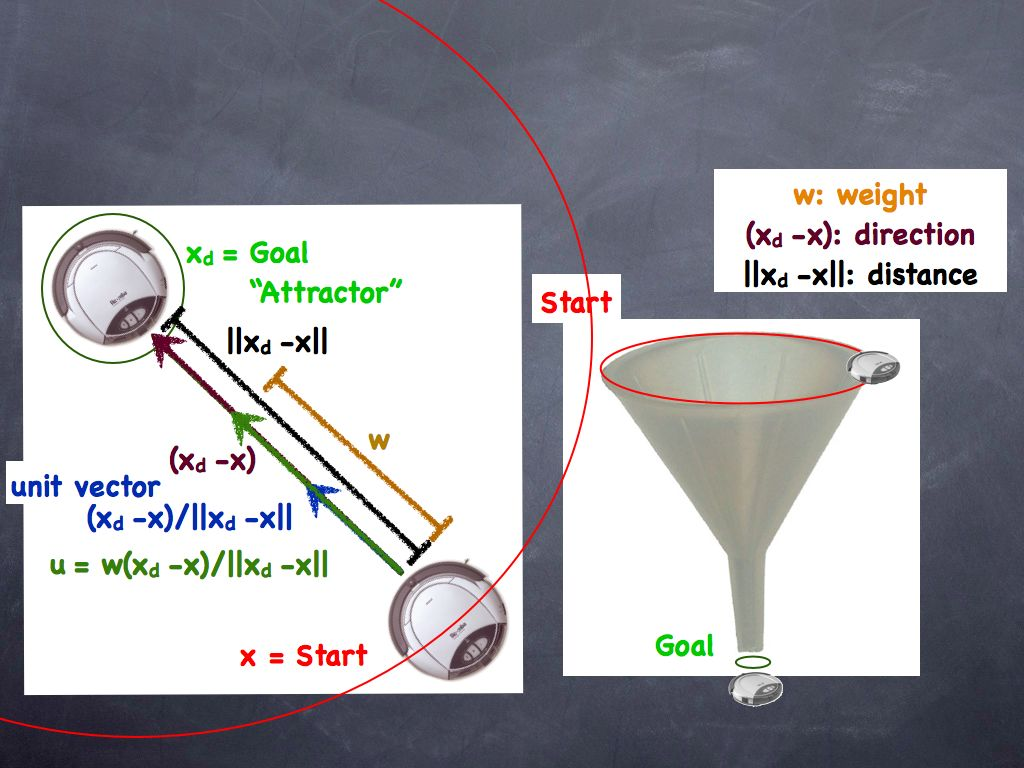
\includegraphics[width=0.6\columnwidth]{figures/7_potential3.jpg}
\caption{``Cone" attractor}
\end{figure}

\begin{figure}[!h]
\centering
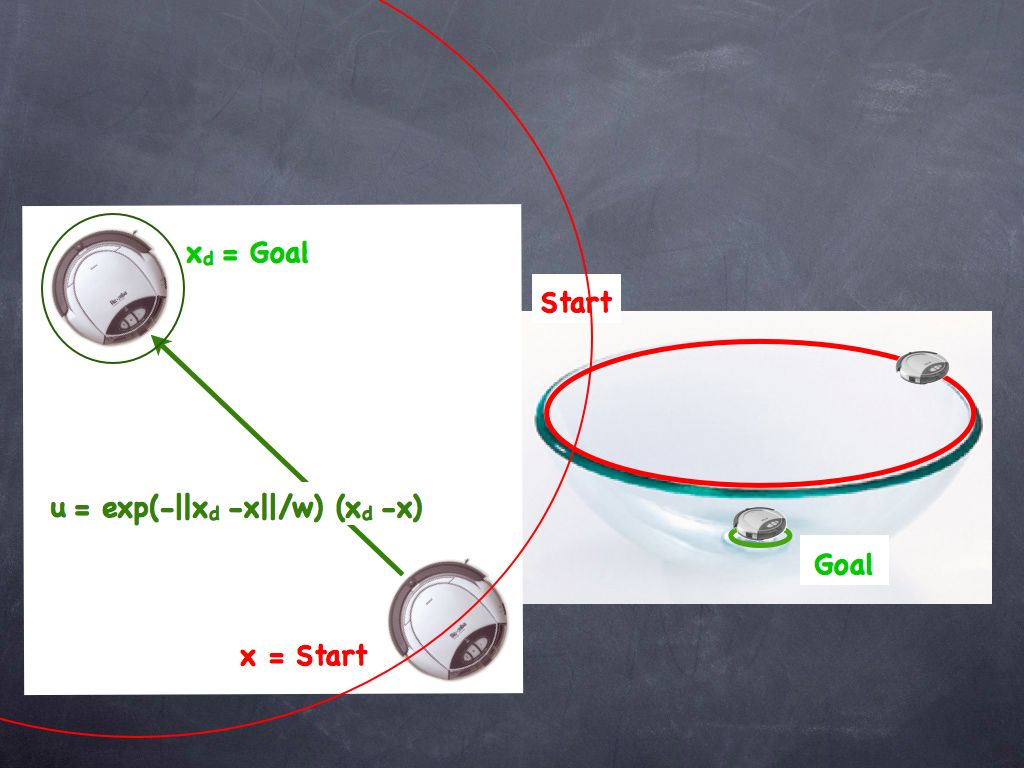
\includegraphics[width=0.6\columnwidth]{figures/7_potential4.jpg}
\caption{``Bowl" attractor}
\end{figure}

\begin{figure}[!h]
\centering
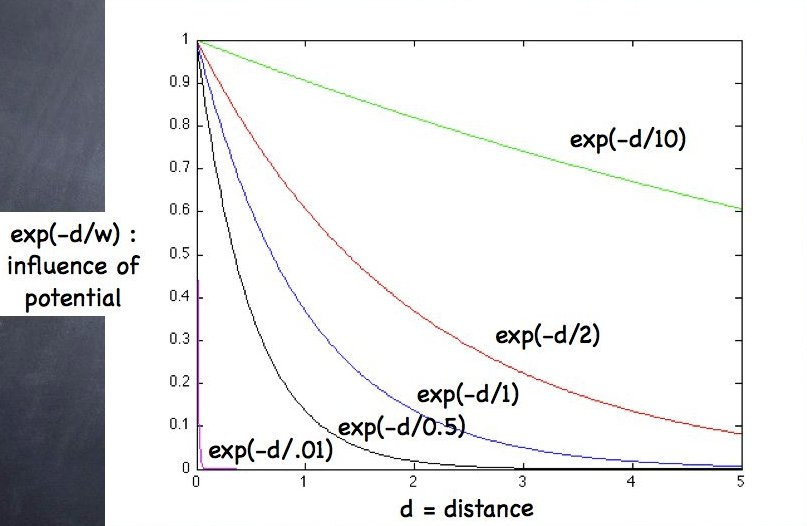
\includegraphics[width=0.6\columnwidth]{figures/7_potential5.jpg}
\caption{exp(-d/w)}
\end{figure}

\begin{figure}[!h]
\centering
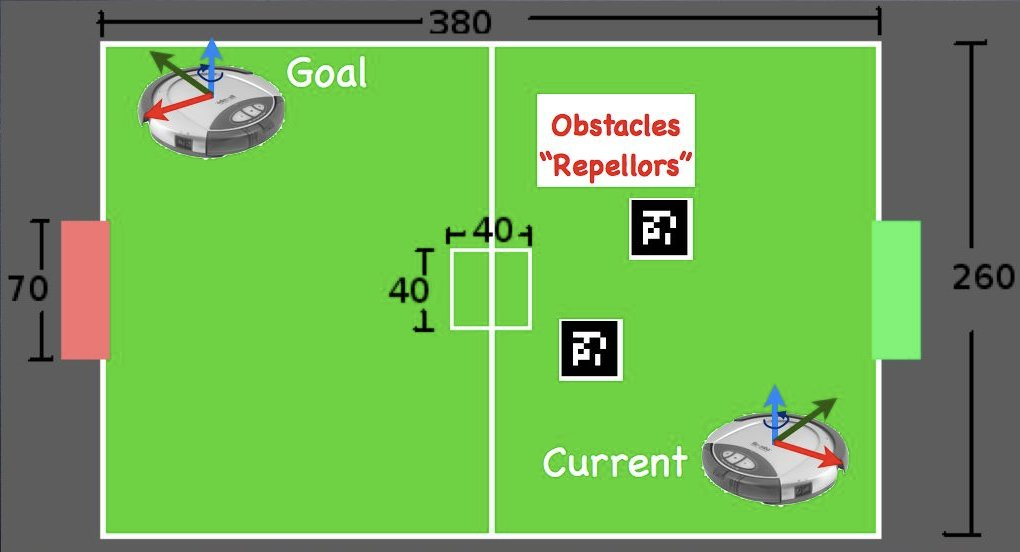
\includegraphics[width=0.6\columnwidth]{figures/7_potential6.jpg}
\caption{Affect of obstacle ``repellors"?}
\end{figure}

\begin{figure}[!h]
\centering
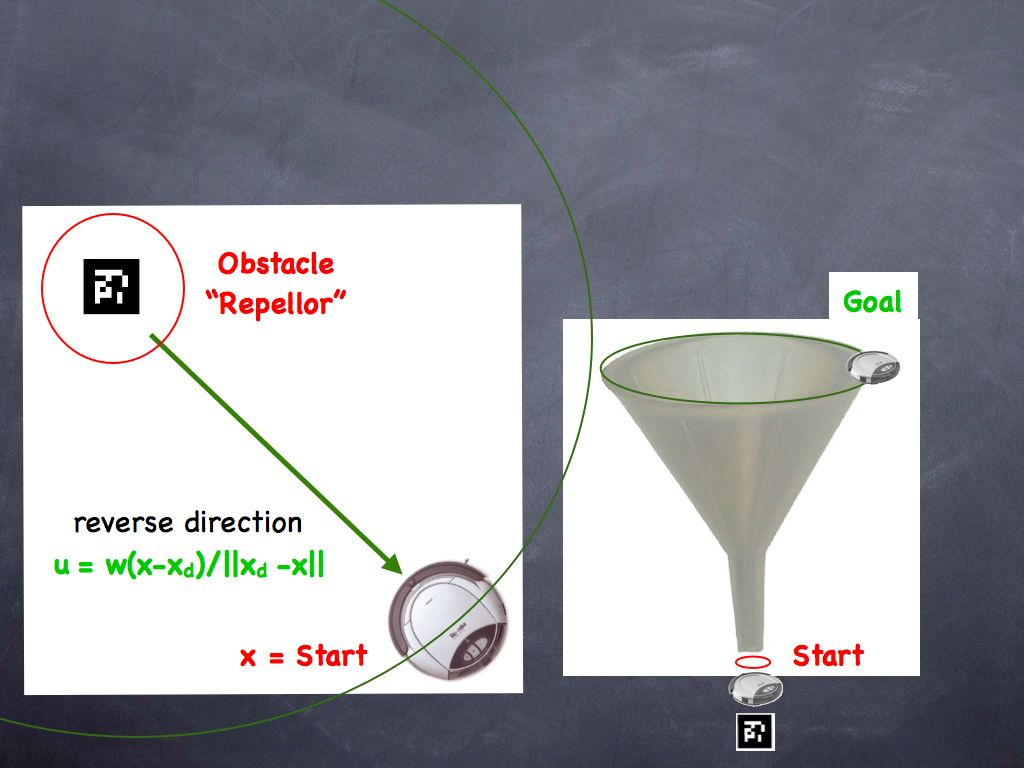
\includegraphics[width=0.6\columnwidth]{figures/7_potential7.jpg}
\caption{``Cone" repellors}
\end{figure}

\begin{figure}[!h]
\centering
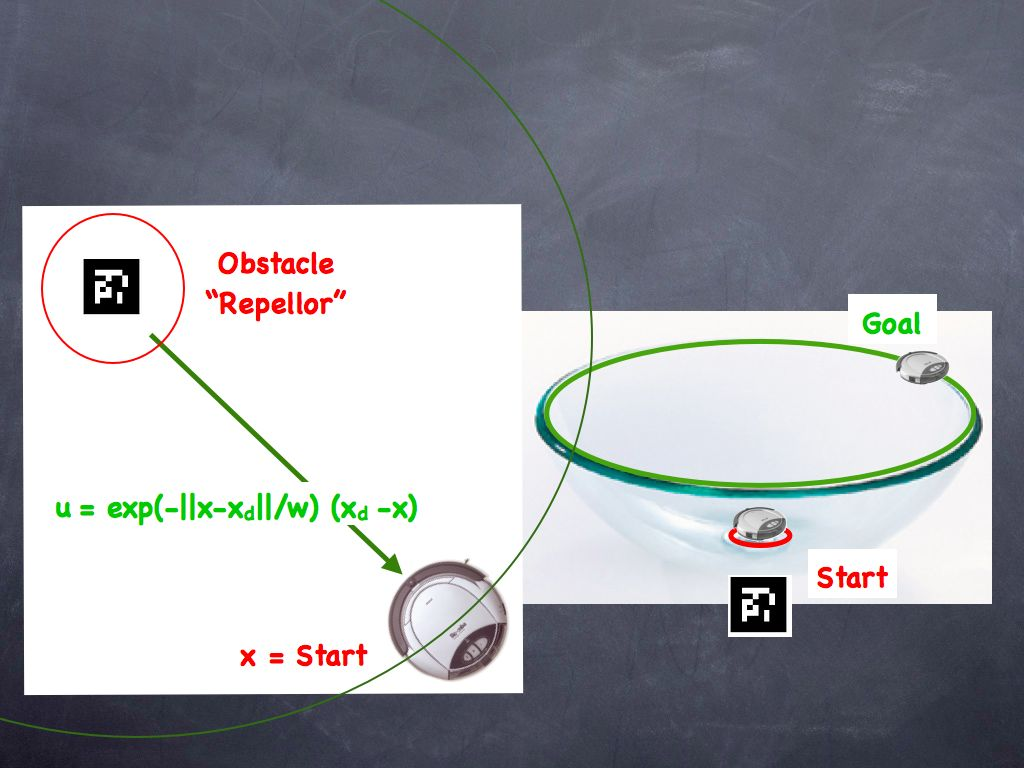
\includegraphics[width=0.6\columnwidth]{figures/7_potential8.jpg}
\caption{``Bowl" repellors}
\end{figure}

link: Potential Fields Matlab Demo

\subsection{Rapidly-exploring Random Trees}

\begin{figure}[!h]
\centering
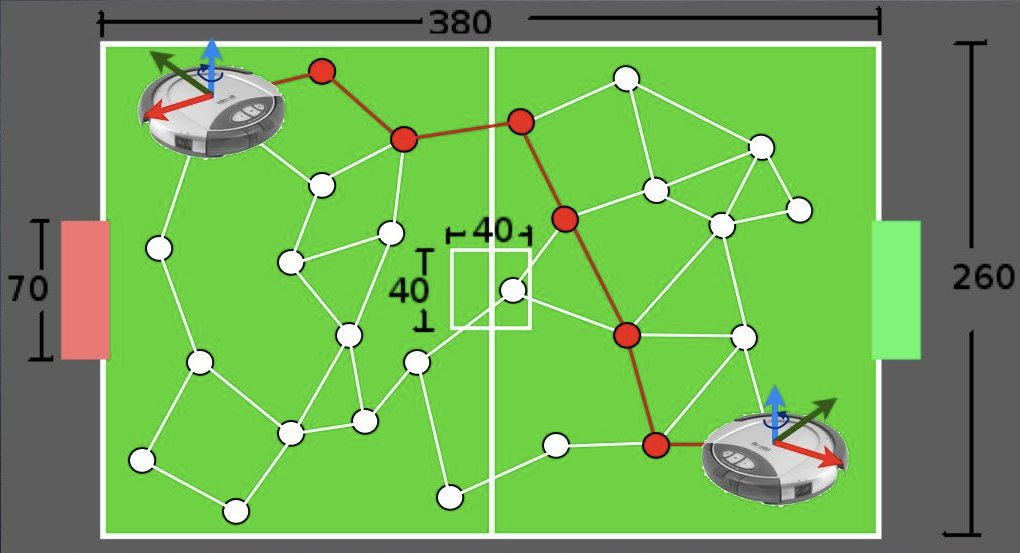
\includegraphics[width=0.6\columnwidth]{figures/7_rrt.jpg}
\caption{RRT}
\end{figure}

\subsection{Probabilistic Road Maps}

\begin{figure}[!h]
\centering
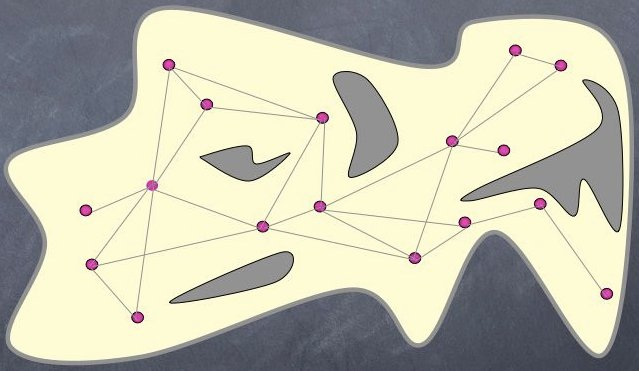
\includegraphics[width=0.6\columnwidth]{figures/7_prm.jpg}
\caption{PRM}
\end{figure}

Given the current starting pose and the goal pose in the soccer field setup, describe the performace of different approaches to path planning are for each of the three cases in Figures \ref{fig:potential9}, \ref{fig:potential10} and \ref{fig:7_potential11}.

\begin{figure}[!h]
\centering
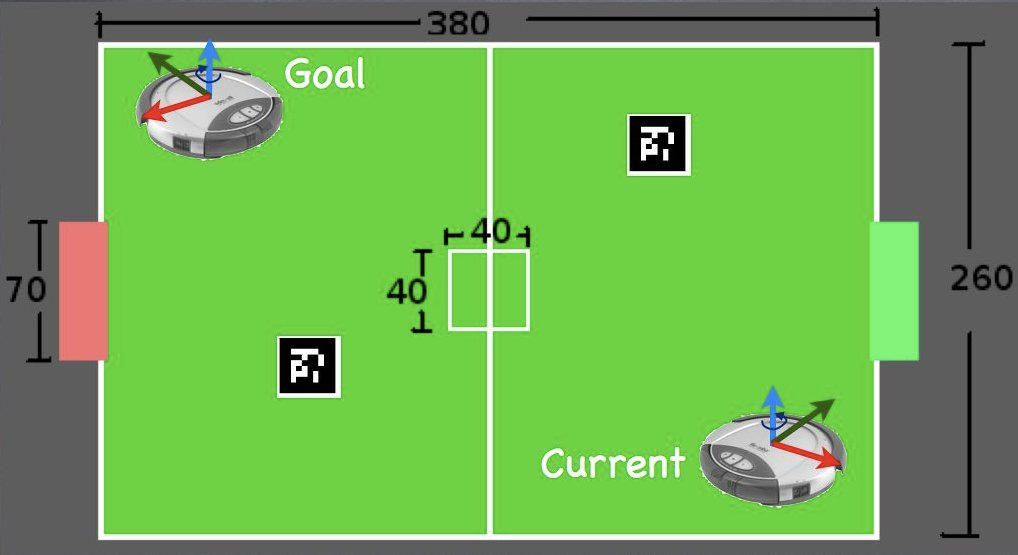
\includegraphics[width=0.6\columnwidth]{figures/7_potential9.jpg}
\label{fig:7_potential9}
\end{figure}

\begin{figure}[!h]
\centering
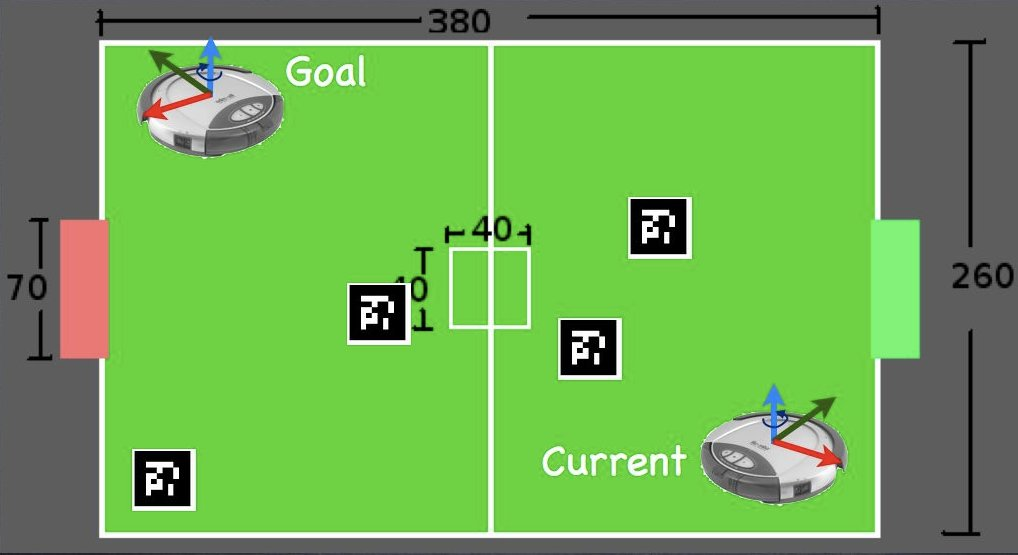
\includegraphics[width=0.6\columnwidth]{figures/7_potential10.jpg}
\label{fig:7_potential10}
\end{figure}

For the case in Figure \ref{fig:potential11}, if using potential fields then the robot will most likely get stuck in a local minima and will never be able to reach the goal pose.

\begin{figure}[!h]
\centering
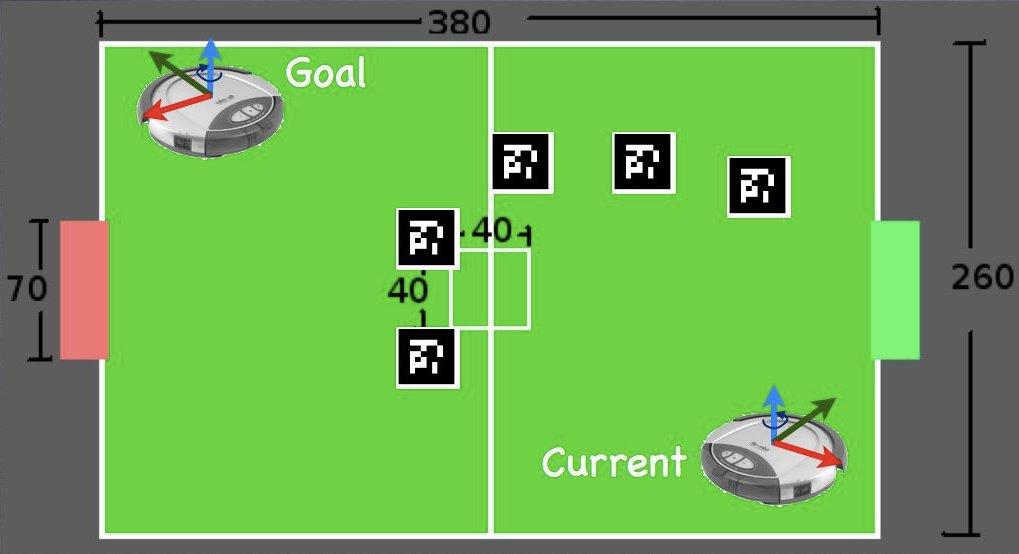
\includegraphics[width=0.6\columnwidth]{figures/7_potential11.jpg}
\label{fig:7_potential11}
\end{figure}


\subsection{Range and Bearing Estimation}

A tutorial on how to determine the difference between a true robot pose and a hypothetical pose

\subsection{Odometry Lab}

\section{Project Infrastructure}

Overhead System; AR tags

\section{Instructions}

\begin{figure}[!h]
\centering
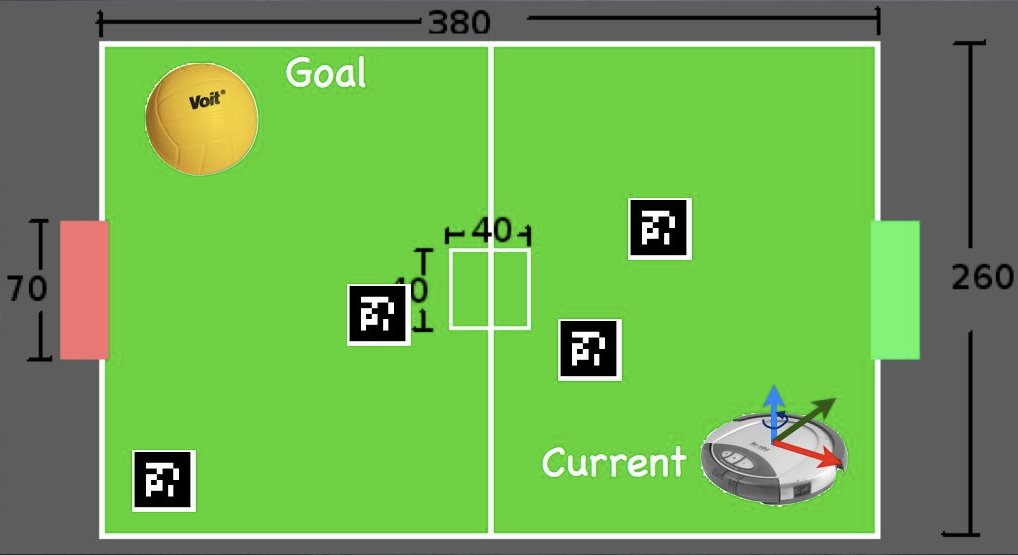
\includegraphics[width=0.6\columnwidth]{figures/7_setup.jpg}
\caption{148 soccer setup}
\end{figure}


\section{Expected Outcomes and Reports}

\vspace{1cm}
\begin{tabular}{|l|l||l|l|}
\hline
{\large \bf Project Implementation} & \\
\hline
\hline
Localization & 5\% \\
$\rightarrow$ Does your robot know where it is given overhead fiducial recognition? & \\
$\rightarrow$ Does your robot know where the goal, the ball, and other players are? & \\
\hline
Goal Attainment  & 15\% \\
$\rightarrow$ Can your robot drive to a given location on the field? & \\
$\rightarrow$ How close to optimal is the robot's path? & \\
$\rightarrow$ How long does it take for your planner to compute? & \\
\hline
Obstacle Avoidance & 15\% \\
$\rightarrow$ Can your robot plan paths in the environment to reach a goal without traversing over obstacles? & \\
$\rightarrow$ Can your robot traverse a given path without hitting objects in the environment? & \\
\hline
Soccer Proficiency & 10\% \\
$\rightarrow$ How well does your robot player soccer in the given environment? & \\
\hline
Controller Robustness & 5\% \\
$\rightarrow$ Does your controller run without interruption? & \\
\hline
\end{tabular}

\newpage
